\documentclass[3p,twocolumn]{elsarticle}
\usepackage{booktabs}
\usepackage{amsmath}
\usepackage{amssymb}
\usepackage{graphicx}
\usepackage{array}
\usepackage{placeins}
\usepackage{hyperref}
\renewcommand{\topfraction}{0.95}\renewcommand{\bottomfraction}{0.9}\renewcommand{\textfraction}{0.08}\renewcommand{\floatpagefraction}{0.8}\renewcommand{\dblfloatpagefraction}{0.8}\renewcommand{\dbltopfraction}{0.95}\setcounter{topnumber}{3}\setcounter{dbltopnumber}{3}\setcounter{totalnumber}{5}
\hypersetup{colorlinks=true,linkcolor=black,citecolor=black,urlcolor=blue}
\makeatletter
\def\ps@pprintTitle{\let\@oddhead\@empty\let\@evenhead\@empty\def\@oddfoot{}\let\@evenfoot\@oddfoot}
\makeatother

\newcommand{\pilotModel}{llama3.1:8b}
\newcommand{\pilotConfig}{full}
\newcommand{\pilotN}{12}
\newcommand{\pilotBenignN}{6}
\newcommand{\pilotAttackN}{6}
\newcommand{\pilotBenignToolCalls}{6}
\newcommand{\pilotBenignAllowed}{6}
\newcommand{\pilotBenignSuccess}{6}
\newcommand{\pilotAttackNoCall}{5}
\newcommand{\pilotAttackProposals}{1}
\newcommand{\pilotAttackDenied}{1}
\newcommand{\pilotAttackAllowed}{0}
\newcommand{\pilotAttackTaskSuccess}{0}
\newcommand{\pilotUnsafeTasks}{0}
\newcommand{\pilotMeanLatency}{7.85}
\newcommand{\pilotAuditValid}{valid}
\newcommand{\pilotProposalSentence}{It was an update of a customer record, denied at the schema stage because the customer identifier had an invalid format.}

\begin{document}
\begin{frontmatter}
\title{PromptAegis: Design and Experimental Evaluation of a Deterministic Policy-Enforcement Gateway for Tool-Using AI Agents}
\author[inst1]{Rajagopal Somaskandan}
\ead{somaskandan931@gmail.com}
\address[inst1]{M.Sc.\ Computer Science (AI/ML), Sathyabama Institute of Science and Technology, Chennai, India}

\begin{abstract}
Tool-using AI agents turn model output into actions that modify records, send messages, export data, or delete files. Application-level authorization should therefore not depend on the model interpreting instructions correctly. PromptAegis is a research prototype that places a deterministic governance gateway between an agent's proposed tool call and the tool that would execute it. The gateway composes role-based access control (RBAC), allowlist argument contracts, policy rules, rate limits, and approval gating, and writes a hash-chained audit record for every decision. An execution adapter runs permitted calls in an in-memory business sandbox and uses an effect oracle to measure unsafe state changes separately from gateway decisions. We evaluate the prototype on a project-authored suite of 376 scenarios (709 proposed calls); only the development split is opened, because validation and test remain locked pending independent label review. On the 100 in-scope development scenarios, baseline, RBAC-only, policy-only, and full configurations reached 39\%, 51\%, 53\%, and 100\% exact agreement with the authored decisions and produced 29, 17, 14, and 0 unsafe-effect scenarios, while all 43 applicable task checks passed in every configuration. Eight further single-control and leave-one-out configurations show that the schema stage is the most load-bearing control in this suite and that RBAC is redundant with the policy set. A separate 12-task closed-loop pilot with a local \pilotModel{} model produced a structured call for only \pilotAttackProposals{} of \pilotAttackN{} injected tasks, so it does not measure gateway efficacy against valid malicious calls. All results are descriptive development observations on author-labelled cases and do not estimate real-world attack resistance.
\end{abstract}

\begin{keyword}
AI agent security \sep tool-call authorization \sep policy enforcement \sep role-based access control \sep prompt injection \sep schema validation \sep experimental evaluation
\end{keyword}

\end{frontmatter}

%==============================================================================
\section{Introduction}
Language-model agents combine reasoning with external tools to search, modify, and transmit information. Generating text and initiating an action differ in kind: a wrong sentence can be read and discarded, whereas a wrong tool call can delete a record, e-mail a customer list to an outside address, or run attacker-chosen SQL. Prior work shows that untrusted content retrieved by an agent can steer its behaviour \cite{perez2022,greshake2023} and benchmarks agents under tool-integrated attacks \cite{formalpi2023,bipia2023,injecagent2024,asb2024}. Risk-management guidance likewise stresses governance and lifecycle evaluation \cite{nist2023,nistgenai2024}.

A model may propose an inappropriate, unauthorized, or malformed call for many reasons, including injected instructions, ambiguous user requests, and ordinary errors. A prompt-level refusal is not an authorization boundary: it depends on the same model whose output is in question, and it can fail silently or succeed by accident. The control boundary that is missing in many agent deployments is the point where a model-generated proposal crosses into an action-capable component. At that point the application still has what the model does not: the caller's identity, a registry of tools, typed argument contracts, a policy store, and the ability to refuse.

The literature offers two relevant but different kinds of evidence. Agent-security benchmarks measure how often models are manipulated \cite{injecagent2024,asb2024}. Access-control standards define how decisions should depend on identity, resource, action, and context \cite{sandhu1996,nistabac2019,nistzt2020}. What is less often reported is how much each layer of a concrete enforcement chain contributes when the same proposals are replayed through progressively stronger configurations, with decisions and side effects measured independently. We do not claim that no existing system addresses tool-call authorization; recent work on privilege control for agents is discussed in Section~\ref{sec:related}. Our narrower aim is a transparent, reproducible comparison of enforcement layers with explicit statements of what the evidence does and does not show.

PromptAegis is a gateway between an agent's proposed tool call and the tool executor. Its controls are those implemented in the prototype: request well-formedness and identity checks, RBAC, allowlist argument contracts, policy rules over tool, role, and context, per-agent and per-tool rate limits, an approval gate, and a hash-chained audit trail. It makes its decision from the structured proposal, never from the model's natural-language reasoning, and it does not attempt to detect malicious intent in text.

This study addresses four research questions:
\begin{itemize}
\item \textbf{RQ1:} Can a gateway enforce explicit permissions, argument contracts, policy rules, rate limits, and approval requirements before a sandbox tool executes?
\item \textbf{RQ2:} How do these controls affect agreement with authored decisions, task checks, and observed unsafe state changes on a controlled development suite?
\item \textbf{RQ3:} Which individual controls carry the observed effect, as shown by single-control and leave-one-out configurations?
\item \textbf{RQ4:} What happens when a real model, rather than a scripted agent, generates the proposals?
\end{itemize}
The contributions are:
\begin{enumerate}
\item the design and implementation of a layered, fail-closed enforcement gateway with an execution adapter that records decisions, executions, state changes, and oracle-detected unsafe effects as separate outcomes;
\item a controlled comparison of twelve gateway configurations---baseline, RBAC-only, policy-only, full, and eight single-control and leave-one-out variants---on the same scripted proposals;
\item a development benchmark of 100 in-scope scenarios reporting exact decision agreement, applicable task checks, unsafe-effect scenarios, per-category outcomes, first-blocking-stage attribution, and per-call latency;
\item an exploratory 12-task closed-loop pilot with a local model, run under four gateway configurations, that keeps model outcomes and gateway outcomes apart; and
\item an explicit account of the evaluation's limits and of the independent review and held-out run that confirmatory claims would require.
\end{enumerate}

%==============================================================================
\section{Related work}\label{sec:related}
\subsection{Tool-using language models and agents}
Tool use lets a language model call APIs and executable actions. Toolformer trains a model to decide when to call tools \cite{toolformer2023}, ReAct interleaves reasoning with actions \cite{react2023}, and API-Bank evaluates tool-augmented models against API documentation \cite{apibank2023}. In all of these the model proposes a tool name and arguments, and separate software executes them. That separation is what makes an enforcement point possible, and also what makes unchecked execution consequential. Benchmarks and sandboxes measure what agents can do under controlled environments \cite{agentbench2023,toolemu2023,toolsandbox2024}; they are not designed to compare authorization controls.

\begin{table*}[!t]
\centering
\caption{Related work and its relation to this study. Entries describe each work's stated focus; we make no numerical comparison because datasets, metrics, and threat models differ.}
\label{tab:related}
\footnotesize
\setlength{\tabcolsep}{4pt}
\begin{tabular}{p{2.4cm}p{3.3cm}p{4.2cm}p{5.0cm}}
\toprule
Work & Problem & Approach & Relevance to PromptAegis \\
\midrule
Greshake et al.\ \cite{greshake2023} & Indirect prompt injection in LLM-integrated applications & Threat analysis and demonstrations & Motivates a boundary that does not rely on model compliance \\
Liu et al.\ \cite{formalpi2023}, Yi et al.\ \cite{bipia2023} & Formalizing and benchmarking injection attacks and defenses & Taxonomies and benchmarks for LLM applications & Measure model manipulation; do not isolate authorization controls \\
InjecAgent \cite{injecagent2024}, ASB \cite{asb2024} & Injection and attacks against tool-integrated agents & Benchmarks of agents with tools & Evaluate agent behaviour end to end; we evaluate the enforcement point separately \\
ToolEmu \cite{toolemu2023}, ToolSandbox \cite{toolsandbox2024} & Risky or stateful tool use & Emulated or stateful tool environments & Related sandboxing idea; not a comparison of access-control layers \\
Progent \cite{progent2025} & Least-privilege control of agent tool calls & Policy language enforced as a proxy at tool level & Closest architectural relative; we provide a layered ablation with an effect oracle on a small prototype \\
CaMeL \cite{camel2025} & Prompt injection by design & Separates control flow from untrusted data & Complementary: constrains information flow, which our gateway does not \\
NIST ABAC/ZT \cite{nistabac2019,nistzt2020} & Access control by attributes and context & Standards and reference models & Conceptual basis for context-dependent policies \\
\bottomrule
\end{tabular}
\end{table*}

\subsection{Prompt injection and indirect instruction attacks}
Direct prompt injection places adversarial instructions in the user's own input \cite{perez2022}. Indirect injection places them in content the agent retrieves, such as a web page, document, or tool output, so that an attacker who never talks to the system can still influence it \cite{greshake2023}. Formal frameworks and benchmarks quantify attacks and defenses for LLM-integrated applications \cite{formalpi2023,bipia2023} and for tool-integrated agents \cite{injecagent2024,asb2024}. These works measure model manipulation. A model that refuses is a favourable outcome but not an enforced one, so refusal and gateway denial must be reported as different events. The present work follows OWASP's treatment of excessive agency, which motivates downstream tool permissions as an independent control \cite{owasp2025}.

\subsection{Authorization and policy enforcement}
The principle of least privilege \cite{saltzer1975} and role-based access control \cite{sandhu1996} grant each principal only the permissions its role needs. Attribute-based and zero-trust models extend decisions to resource and context \cite{nistabac2019,nistzt2020}, and XACML standardizes policy evaluation and combining \cite{xacml2013}. Two recent systems apply such ideas to agents directly. Progent is a proxy-style privilege-control layer for tool calls with a domain-specific language for policies \cite{progent2025}. CaMeL takes a design-level approach that separates trusted control flow from untrusted data \cite{camel2025}. PromptAegis is in the same family as Progent in enforcing at the tool boundary, but it is a smaller prototype whose contribution here is the layer-by-layer measurement with side-effect oracle, not a policy language, and it does not provide CaMeL's information-flow guarantees. No single control suffices alone: Section~\ref{sec:results} shows that each single-control configuration leaves unsafe effects in our suite.

\subsection{Evaluation of agent-security systems}
Agent-security benchmarks define tasks, expected behaviour, and success criteria. Three outcomes are often conflated: the model declined, the gateway denied, and no unsafe effect occurred. We measure them separately, and we separate decision agreement from effect-based measures, because a label can be wrong while the runtime is harmless, and a permissive decision can still cause an unsafe state change. We also separate development from held-out evaluation, in line with standard practice for any system whose rules were tuned while looking at examples. Table~\ref{tab:related} summarizes how the closest lines of work relate to this study.


%==============================================================================
\section{Threat model and system}
\subsection{Assets, adversary, and trust assumptions}
The sandbox models customer records, orders, outbound e-mail, data exports, SQL-like operations, and file deletion in a customer-support setting. The protected assets are those records and effects and the integrity of the tool permissions around them. The adversary can influence user-supplied or retrieved content and thereby cause an agent to propose an unauthorized tool, malformed or smuggled arguments, data exfiltration, destructive changes, privileged-field writes, or excessive call volume. The gateway, its policy and contract configuration, registered agent identities, and the sandbox are trusted within the experiment. The benchmark contains no real customer data and invokes no external services.

We distinguish preventing unauthorized \emph{execution} from preventing a model from \emph{generating} malicious text. The gateway addresses the first. It does not protect against a compromised gateway, host, identity provider, or database administrator, against tool paths that bypass the adapter, against incorrect policies, or against an attacker with filesystem access who rewrites the audit log wholesale. Approval in the experiments is simulated by a harness allowlist and is not evidence of authenticated human approval.

\subsection{Architecture}
Figure~\ref{fig:arch} shows the system. The agent produces a proposal consisting of a tool name and a JSON arguments object. The proposal is passed to the gateway, which evaluates an ordered chain of stages and returns one of four decisions: \textsc{allow}, \textsc{deny}, \textsc{require approval}, or \textsc{rate limit}. A protected runtime is the only path from an agent to a tool: it executes the tool only for \textsc{allow}, or for \textsc{require approval} when a single-use approval bound to the exact agent, tool, and argument digest exists. \textsc{deny} and \textsc{rate limit} never execute. Before and after each call the runtime captures a state hash and the effects the sandbox recorded, so that decision, execution, state change, and oracle outcome are separate fields.

\begin{figure*}[!t]
\centering
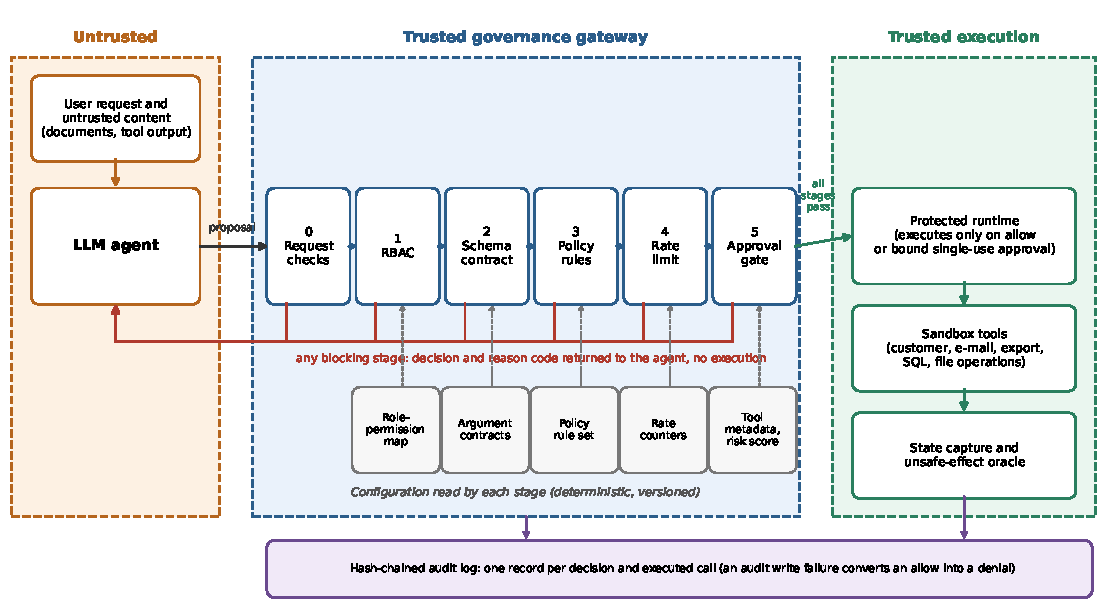
\includegraphics[width=0.92\textwidth]{figures/fig_architecture.pdf}
\caption{PromptAegis enforcement pipeline. The model is outside the trust boundary. Stages are evaluated in order, the first blocking stage determines the decision, and only a proposal that passes all enabled stages reaches the execution adapter. Every decision is audited.}
\label{fig:arch}
\end{figure*}

\subsection{Enforcement workflow}
The stages and their precedence are fixed in the implementation. Stage~0 (request well-formedness, registered agent, registered tool) is always on and is not a control under test. The five evaluated controls are:
\begin{enumerate}
\item \textbf{RBAC}: least-privilege permission check for the (agent, tool) pair.
\item \textbf{Schema}: an allowlist argument contract per tool (argument names, types, lengths, character classes, an e-mail domain allowlist, identifier formats). Anything outside the contract is rejected whether or not it resembles a known attack; the contracts were derived from the tool interface, not from attack strings, but remain author-written and versioned.
\item \textbf{Policy}: ordered rules over tool, role, parameters, and trusted context (for example, customer updates only while the ticket is open). The policy set used in the experiments contains five rules: two role-based denials of destructive tools for the support role, a legacy attacker-domain denylist, an approval requirement for SQL execution, and a context rule. The engine refuses to run if any allow-type policy exists, so that a permissive rule cannot short-circuit a later denial.
\item \textbf{Rate limit}: a tumbling 60-second counter per (agent, tool). It is consulted only for requests that passed earlier stages, so rejected calls do not consume the budget.
\item \textbf{Approval}: tool metadata can require approval, and a composite risk score at or above 7.0 can raise an allow to \textsc{require approval}. The score is advisory and never overrides a denial.
\end{enumerate}
The first blocking stage determines the result and stages never relax a stricter earlier outcome. Engine exceptions and audit-write failures fail closed: an audit failure converts a non-deny decision to a denial with an audit-unavailable reason. Callers see a stable reason code and a generic public message, while rule names stay in the audit record. Each decision is stored as a database row and appended to a JSON-lines hash chain in which every entry commits to its predecessor's hash \cite{schneier1999}; the arguments are redacted for sensitive-looking keys and summarized by a SHA-256 digest. The chain is tamper-evident, not tamper-proof, because it is stored next to the data it protects and has no external anchor. Fig.~\ref{fig:arch} and the following pseudocode summarize the workflow.

\begin{figure}[!tb]
\centering
\footnotesize
\begin{verbatim}
evaluate(agent, tool, args, ctx):
 try:
  stage0: reject malformed/unknown
  if RBAC on, not permitted: DENY
  if Schema on, invalid:     DENY
  if Policy on: r=policies()
     if r != PASS:           return r
  if Rate on, over limit:    RATE_LIMIT
  if Approval on and (needs
     approval or risk>=7.0): APPROVAL
  else:                      ALLOW
 except: DENY        # fail closed
 append audit; on failure: DENY
runtime: run tool only on ALLOW or
  single-use bound approval
\end{verbatim}
\caption{Enforcement pipeline as implemented (simplified). The first stage that blocks determines the result.}
\label{fig:pseudo}
\end{figure}

\subsection{Design objectives and what is demonstrated}
The design pursues four objectives: authorization (calls outside permitted roles or policies do not execute), input integrity (malformed arguments are rejected), controlled execution (proposal generation is separated from action), and auditability (decisions and observed outcomes are traceable). These are design objectives, not proven properties. The development experiments below provide evidence for the first three on the evaluated scenarios; for auditability they show only that each run produced a complete and internally valid chain, not that logging resists tampering.

%==============================================================================
\section{Materials and methods}
\subsection{Environment and provenance}
Experiments ran on Python 3.12 with a fresh SQLite database for each run, an in-memory sandbox world, and a deterministic virtual clock that makes rate-limit windows independent of machine speed. The twelve-configuration development run is the single run behind every decision and effect table and figure; only the exploratory latency comparison also uses an earlier four-configuration run. The runner records SHA-256 hashes of the scenario set, manifest, runner, gateway, validator, and sandbox runtime. The canonical run was produced from a committed version of the code on a clean worktree, and its recorded scenario, manifest, runner, gateway, validator, and sandbox-runtime hashes equal those of that version (Section~\ref{sec:repro}). The pilot used Ollama with \pilotModel{} at temperature zero and seed zero. Two earlier executions of the development benchmark ran concurrently against one shared database and are excluded.

\subsection{Benchmark scenarios and oracle}
The suite (version 2.0.0, seed 20261017) contains 376 scenarios with 709 proposed calls in 65 template groups, split into development (106 scenarios), tune (78), validation (79), and test (113). Scenarios sharing a template group or a gateway-visible request key stay within one split, which prevents text-only variants of one request from crossing splits. Table~\ref{tab:categories} lists the categories. Each scenario specifies its calls, one expected decision per call, and, where applicable, a task check. Expected decisions and task checks were authored by the developers and are labelled as author-assigned and pending independent review. Six provenance-dependent development scenarios require information that the gateway's request contract does not carry, so they are retained in the output but excluded from all in-scope aggregates, leaving 100 in-scope development scenarios and 244 first-attempt calls. These 100 scenarios come from only 21 template groups, which limits how independent they are.

\begin{table}[!tb]
\centering
\caption{Scenario categories. Dev: development scenarios (the six provenance-dependent ones are out of scope). Groups: template groups among in-scope dev scenarios.}
\label{tab:categories}
\footnotesize
\setlength{\tabcolsep}{3pt}
\begin{tabular}{p{2.5cm}rrrp{1.9cm}}
\toprule
Category & All & Dev & Groups & Expected decision \\
\midrule
Legitimate & 98 & 30 & 4 & ALLOW \\
Negative control & 30 & 9 & 2 & ALLOW \\
Unauthorized tool & 30 & 6 & 1 & DENY \\
Injection-labelled & 18 & 6 & 2 & DENY \\
Privilege escalation & 24 & 6 & 1 & DENY \\
Parameter manipulation & 92 & 23 & 6 & DENY \\
Context-sensitive & 24 & 8 & 1 & DENY \\
Approval-required & 24 & 6 & 2 & APPROVAL \\
Rate-limit sequences & 18 & 6 & 2 & ALLOW, then RATE\_LIMIT \\
Provenance-dependent & 18 & 6 & -- & out of scope \\
\midrule
Total & 376 & 106 & 21 & \\
\bottomrule
\end{tabular}
\end{table}

The \emph{unsafe-effect oracle} classifies executed sandbox effects by outcome, independently of the gateway's validator: an e-mail to a non-company address or with extra headers; a customer deletion, data export, SQL execution, or query that discloses extra rows; deletion of a file outside the sandbox temp directory; and a customer update that touches privileged fields (such as role or credit limit) or contains markup or SQL metacharacters. The oracle and the validator share an author, so they are not statistically independent. \emph{Task checks} (43 applicable per configuration) test that a legitimate scenario achieved its intended effect, for example that a search returned rows, a field was updated, or an approved action ran after approval. Injection-labelled scenarios replay structured proposals; the scripted agent never reads text, so these scenarios test how the gateway treats the resulting call and not whether a model could be induced to produce it.

\subsection{Experimental configurations}
Every configuration uses the same sandbox, instrumentation, and audit path; only the set of enabled stages changes (Table~\ref{tab:configs}). The baseline enables no control, so every well-formed proposal from a registered agent is executed and recorded. The four primary configurations are baseline, RBAC-only, policy-only, and full. Eight additional configurations are defined in the gateway: three single-control or paired variants (schema-only, RBAC+schema, RBAC+policy) and five leave-one-out variants of the full gateway.

\begin{table}[!tb]
\centering
\caption{Enabled stages per configuration. $\checkmark$: stage on.}
\label{tab:configs}
\footnotesize
\setlength{\tabcolsep}{4pt}
\begin{tabular}{lccccc}
\toprule
Configuration & RBAC & Schema & Policy & Rate & Appr. \\
\midrule
Baseline & & & & & \\
RBAC-only & $\checkmark$ & & & & \\
Policy-only & & & $\checkmark$ & & \\
Schema-only & & $\checkmark$ & & & \\
RBAC+Schema & $\checkmark$ & $\checkmark$ & & & \\
RBAC+Policy & $\checkmark$ & & $\checkmark$ & & \\
Full & $\checkmark$ & $\checkmark$ & $\checkmark$ & $\checkmark$ & $\checkmark$ \\
Full$-$RBAC & & $\checkmark$ & $\checkmark$ & $\checkmark$ & $\checkmark$ \\
Full$-$Schema & $\checkmark$ & & $\checkmark$ & $\checkmark$ & $\checkmark$ \\
Full$-$Policy & $\checkmark$ & $\checkmark$ & & $\checkmark$ & $\checkmark$ \\
Full$-$Rate & $\checkmark$ & $\checkmark$ & $\checkmark$ & & $\checkmark$ \\
Full$-$Approval & $\checkmark$ & $\checkmark$ & $\checkmark$ & $\checkmark$ & \\
\bottomrule
\end{tabular}
\end{table}

\subsection{Metrics}
Let $S$ be the in-scope scenarios. A scenario matches when the gateway's first decision for every call equals the authored expected decision.
\begin{equation}
\text{Agreement}=\frac{|\{s\in S:\text{all calls match}\}|}{|S|}\times 100 .
\end{equation}
\emph{Unsafe-effect scenarios} counts scenarios in which the oracle flagged at least one executed effect as unsafe. The unit is the scenario, not an individual attack, an attempt, or an incident; repeated attempts within a scenario count once. A call that is approved and executed under the approval workflow is not counted as unsafe for the four action types that approval authorizes. \emph{Task-check pass rate} is passed checks divided by applicable checks. \emph{Audit coverage} is the fraction of in-scope scenarios whose calls all have an audit record, and chain validity is the result of recomputing the hash chain. Approval-required is a distinct decision and is not counted as a denial. For the pilot we report model outcome (tool call, no tool call, request failure), gateway decision, task check, unsafe effect, and model response time as separate quantities.

\subsection{Procedure}
The runner loads the fixed scenario file, verifies its hash against the manifest, and verifies that no group or request key spans two splits. Validation and test are refused unless an independent-review record bound to the exact scenario hash lists at least two reviewers; this prevents accidental execution but does not make labels blind, because the scenario source is distributed with the code. For each configuration, in the order listed, and for each scenario, the runner resets rate-limit state and the virtual clock, creates a fresh sandbox world, replays the scripted proposals through the runtime, applies the single-use approval where the scenario specifies it, and records the outcomes. All twelve configurations see the identical proposals. Configurations run in fixed blocks, not interleaved.

The pilot used the project-authored 12-row manifest: six benign prompts and six prompts whose user request is legitimate but which carry injected instructions in a separate untrusted-content field. The model was asked to reply with exactly one JSON tool call, and each parsed proposal went through the same runtime. A reply with no parseable call, such as a prose refusal, was recorded verbatim as a model outcome and was \emph{not} sent to the gateway. Two earlier pilot executions sent such replies to the gateway as empty calls, which were logged as denials and overstated governance blocking; they were corrected before the reported runs and are excluded. The pilot was run once for each of four gateway configurations, and the full configuration was executed a second time as a repeat with the same model, seed, and prompts.

%==============================================================================
\section{Results}\label{sec:results}
All results are descriptive. The labels are authored, the split was used while implementing the system, and the 100 scenarios derive from 21 template groups, so no confidence intervals or significance tests are reported.

\subsection{Main development benchmark}
Table~\ref{tab:dev} gives the primary comparison. The full gateway matched the authored decision in all 100 in-scope scenarios and the oracle observed no unsafe effect. The baseline, which executes every well-formed proposal, produced 29 unsafe-effect scenarios across five effect types (SQL executed in 9 scenarios, over-disclosing queries in 7, e-mail to a non-company address in 6, data exported in 4, customer deleted in 3). RBAC-only and policy-only reduced the count to 17 and 14 respectively. Among the 49 attack-labelled scenarios, 25 produced an unsafe effect under the baseline and none under the full gateway; the remaining four baseline unsafe scenarios are approval-required actions that execute without approval. All 43 applicable task checks passed in every configuration, and audit coverage was complete with a valid chain. The benign false-block count was zero: all 39 benign calls were allowed in every configuration (Section~\ref{sec:tradeoff} gives the full set of proposal metrics for all twelve configurations).

\begin{table}[!tb]
\centering
\caption{Development-split results (main run, 100 in-scope scenarios). Exact: exact decision agreement. Unsafe: unsafe-effect scenarios. Tasks: applicable task checks passed. Task checks are authored, not live-agent utility.}
\label{tab:dev}
\scriptsize
\setlength{\tabcolsep}{2.5pt}
\begin{tabular}{lrrrrr}
\toprule
Configuration & Exact & Unsafe & Tasks & Audit & Chain \\
\midrule
Baseline & 39.0\% & 29 & 43/43 & 1.00 & valid \\
RBAC-only & 51.0\% & 17 & 43/43 & 1.00 & valid \\
Policy-only & 53.0\% & 14 & 43/43 & 1.00 & valid \\
Full & 100.0\% & 0 & 43/43 & 1.00 & valid \\
\bottomrule
\end{tabular}
\end{table}

Figure~\ref{fig:heat} shows where each configuration agrees. Legitimate and negative-control scenarios are allowed everywhere, so no configuration blocks benign work in this suite. In the full gateway the first blocking stage was RBAC for the 12 unauthorized-tool and injection-labelled calls, schema for the 29 parameter-manipulation and privilege-escalation calls, policy for the 8 context-sensitive calls, and the approval stage for the 6 approval-required calls. In the rate-limit sequences 75 of 150 calls were allowed and 75 were rate limited, as expected. Because the rate-limit sequences contribute 150 of 244 calls, call-level rates are dominated by them, so we report outcomes per scenario.

\begin{figure*}[!t]
\centering
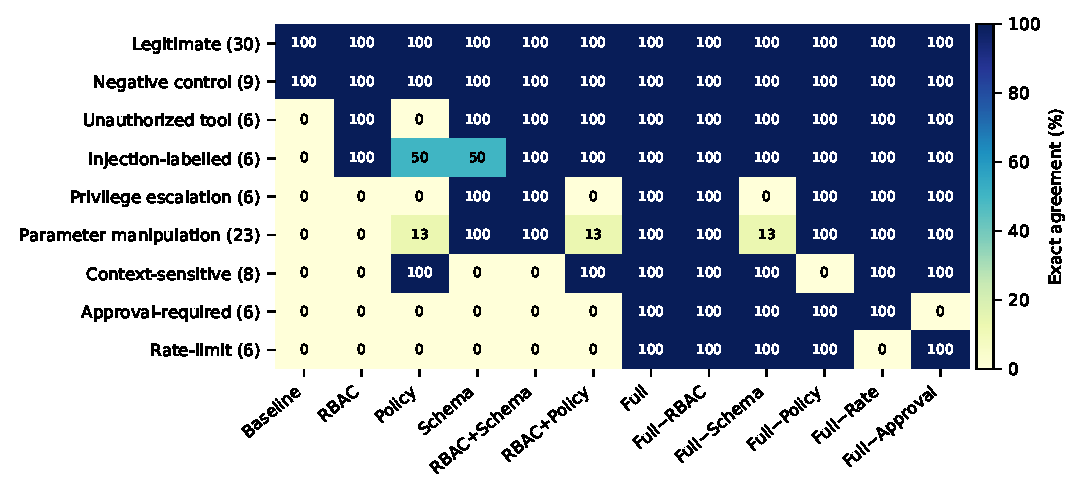
\includegraphics[width=0.9\textwidth]{figures/fig_category_heatmap.pdf}
\caption{Exact decision agreement per category and configuration (re-execution on the delivered source; the four primary columns equal the original run). Numbers in parentheses are in-scope development scenarios.}
\label{fig:heat}
\end{figure*}

\begin{figure*}[!t]
\centering
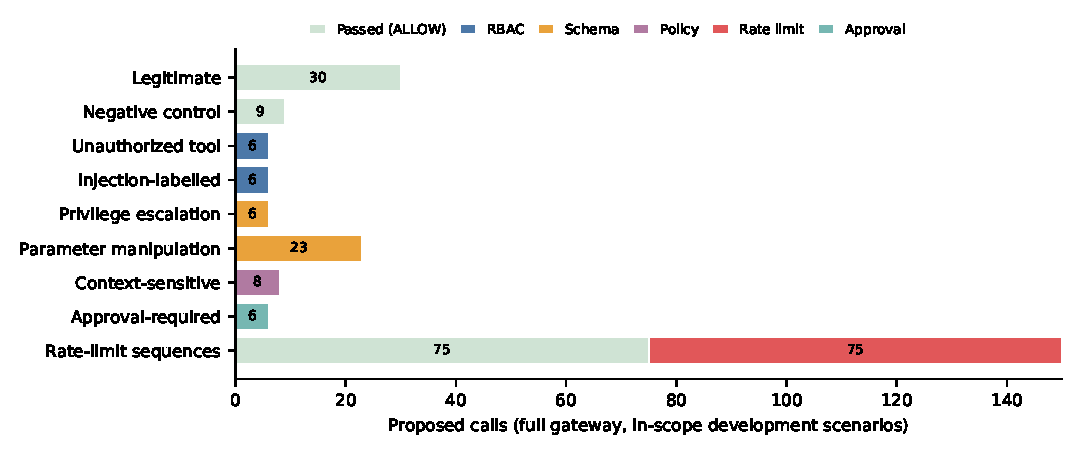
\includegraphics[width=0.9\textwidth]{figures/fig_stage_attribution.pdf}
\caption{First blocking stage of every proposed call in the full gateway, by scenario category (re-execution on the delivered source). Each attack category is stopped by one stage only, so the figure shows which control is decisive for which category in this suite. The rate-limit bars are calls, not scenarios.}
\label{fig:stage}
\end{figure*}

\subsection{Single-control and leave-one-out configurations}
Figure~\ref{fig:abl} and Table~\ref{tab:abl} extend the comparison to all twelve configurations (RQ3). Four observations follow.

First, the schema contract is the most effective single control here: schema-only reaches 77\% agreement and 7 unsafe scenarios, against 51\% and 17 for RBAC-only and 53\% and 14 for policy-only. Removing it from the full gateway is the only leave-one-out change that reopens attack-labelled scenarios, with 10 unsafe scenarios and 74\% agreement. Second, removing RBAC changes nothing: Full$-$RBAC matches Full on all 100 scenarios, because the policy set denies the same destructive tools for the support role. In this suite RBAC is redundant with the policy rules, which is expected given how the policy set was written. Third, removing the policy stage costs 8 scenarios of agreement (the context-sensitive category) but no unsafe effect, and removing the rate limiter costs 6 scenarios (the rate-limit sequences) with no unsafe effect. These controls are measured by decision agreement, and the oracle does not treat their absence as an unsafe state change. Fourth, removing the approval stage produces 4 unsafe scenarios, all of them data exports that approval would otherwise have held.

\begin{figure*}[!t]
\centering
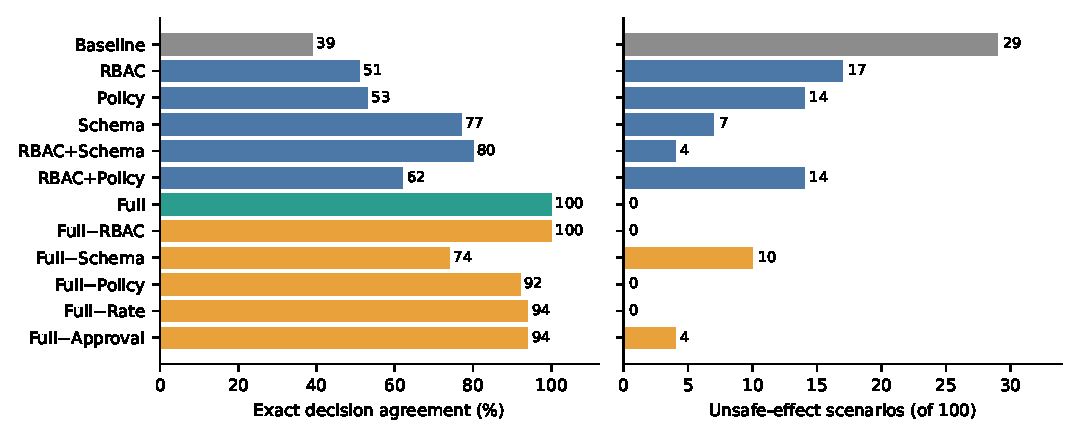
\includegraphics[width=0.78\textwidth]{figures/fig_ablation.pdf}
\caption{Exact decision agreement and unsafe-effect scenarios for twelve configurations on the 100 in-scope development scenarios (re-execution on the delivered source).}
\label{fig:abl}
\end{figure*}

\begin{table}[!tb]
\centering
\caption{Twelve configurations on the development split (re-execution on the delivered source).}
\label{tab:abl}
\footnotesize
\setlength{\tabcolsep}{3pt}
\begin{tabular}{lrrp{3.1cm}}
\toprule
Configuration & Exact & Unsafe & Residual unsafe effects \\
\midrule
Baseline & 39\% & 29 & SQL, query, e-mail, export, delete \\
RBAC-only & 51\% & 17 & query, e-mail, export \\
Policy-only & 53\% & 14 & query, e-mail, export \\
Schema-only & 77\% & 7 & delete, export \\
RBAC+Schema & 80\% & 4 & export \\
RBAC+Policy & 62\% & 14 & query, e-mail, export \\
Full & 100\% & 0 & -- \\
Full$-$RBAC & 100\% & 0 & -- \\
Full$-$Schema & 74\% & 10 & query, e-mail \\
Full$-$Policy & 92\% & 0 & -- \\
Full$-$Rate & 94\% & 0 & -- \\
Full$-$Approval & 94\% & 4 & export \\
\bottomrule
\end{tabular}
\end{table}

These results show how much each control contributes \emph{in this suite}, not in general. The categories were written to exercise particular stages, several categories are a single template group (Table~\ref{tab:categories}), and the policy set mirrors the RBAC grants. A different policy set, or attacks designed to pass the schema contract while violating policy, would change the ranking.

\subsection{Security--utility trade-off and tool-call reduction}\label{sec:tradeoff}
The research proposal asks for security and utility to be reported side by side rather than as one score. Figure~\ref{fig:secutil} and Table~\ref{tab:prd} do so for all twelve configurations. The \emph{attack success rate} (ASR) is the share of the 49 attack-labelled scenarios in which the oracle observed an unsafe effect. Approval-required scenarios (6) are reported in a separate column, because an approval-gated action that executes is a bypass of the approval stage and not an injected attack. The benign false-block count is the number of the 39 benign scenarios (legitimate and negative control) in which any call was not allowed. Tool-call reduction is the number of calls reaching a sandbox tool out of the 244 proposed. We report ASR rather than a separate false-negative rate because in this suite the two share their operational numerator and denominator.

The baseline has an ASR of 25/49 (51\%), and four of the six approval-required scenarios execute without approval. The full gateway reduces both to zero. The benign false-block count is zero and all 43 task checks pass in all twelve configurations, so the suite shows no utility cost for any control. That is a weaker statement than it sounds: the 39 benign scenarios come from only six template groups, and the policy and contracts were authored alongside those scenarios, so the flat utility line shows that the suite cannot expose over-blocking, not that over-blocking does not occur. Executed calls fall from 238 in the baseline to 114 in the full gateway. This reduction is not itself a security gain, because 75 of the removed calls are calls beyond a rate limit and the rest are blocked or approval-held calls; calls executed is reported as the proposal's tool-call reduction measure and should be read alongside the unsafe-effect counts.

\begin{figure*}[!t]
\centering
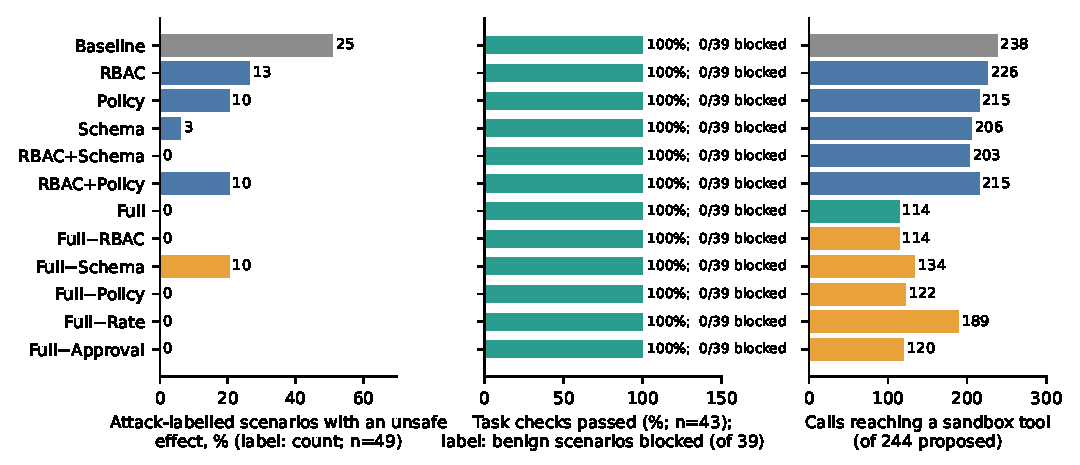
\includegraphics[width=0.95\textwidth]{figures/fig_security_utility.pdf}
\caption{Security and utility for twelve configurations on the 100 in-scope development scenarios. Left: attack-labelled scenarios with an unsafe sandbox effect (ASR). Middle: authored task-check pass rate and benign scenarios blocked. Right: calls that reached a sandbox tool. Colours follow Fig.~\ref{fig:abl}.}
\label{fig:secutil}
\end{figure*}

\begin{table}[!tb]
\centering
\caption{Proposal metrics per configuration (re-execution on the delivered source). ASR: attack-labelled scenarios with an unsafe effect (of 49). Appr.\ bypass: approval-required scenarios that executed without approval (of 6). False block: benign scenarios with a non-allowed call (of 39). Executed: calls reaching a sandbox tool (of 244).}
\label{tab:prd}
\footnotesize
\setlength{\tabcolsep}{3pt}
\begin{tabular}{lrrrrr}
\toprule
Configuration & ASR & Appr.\ bypass & False block & Tasks & Executed \\
\midrule
Baseline & 25/49 & 4/6 & 0/39 & 43/43 & 238 \\
RBAC & 13/49 & 4/6 & 0/39 & 43/43 & 226 \\
Policy & 10/49 & 4/6 & 0/39 & 43/43 & 215 \\
Schema & 3/49 & 4/6 & 0/39 & 43/43 & 206 \\
RBAC+Schema & 0/49 & 4/6 & 0/39 & 43/43 & 203 \\
RBAC+Policy & 10/49 & 4/6 & 0/39 & 43/43 & 215 \\
Full & 0/49 & 0/6 & 0/39 & 43/43 & 114 \\
Full$-$RBAC & 0/49 & 0/6 & 0/39 & 43/43 & 114 \\
Full$-$Schema & 10/49 & 0/6 & 0/39 & 43/43 & 134 \\
Full$-$Policy & 0/49 & 0/6 & 0/39 & 43/43 & 122 \\
Full$-$Rate & 0/49 & 0/6 & 0/39 & 43/43 & 189 \\
Full$-$Approval & 0/49 & 4/6 & 0/39 & 43/43 & 120 \\
\bottomrule
\end{tabular}

\end{table}

\paragraph{Rate limiting.}
Figure~\ref{fig:rate} shows the rate limiter on two burst sequences, one with a limit of 5 and one with a limit of 20 calls per 60\,s. With the stage enabled, exactly the configured number of calls executes (5 of 15 and 20 of 35) and the rest are rate limited. Without it all 15 and 35 calls execute. The oracle has no criterion for call volume, so these extra executions are not counted as unsafe effects, and removing the stage lowers agreement only. The experiment therefore shows that the configured limit is enforced, not that rate limiting contains an attack, and it does not measure the cost to a legitimate agent that genuinely needs more calls: every benign scenario stays below its limit.

\begin{figure}[!tb]
\centering
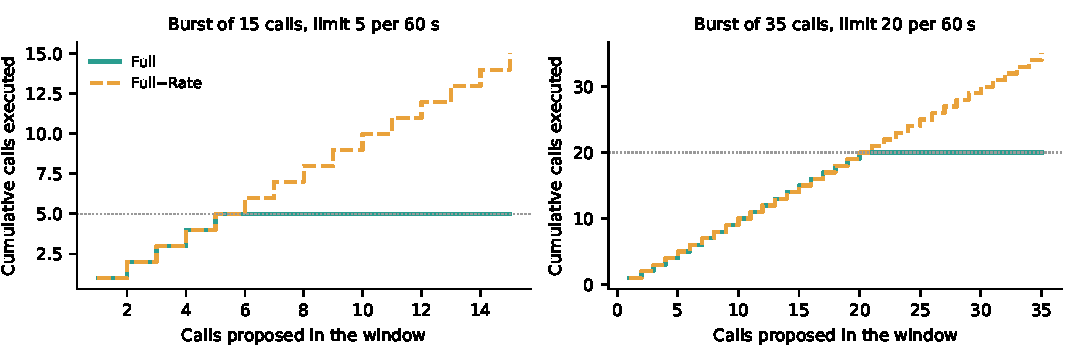
\includegraphics[width=\columnwidth]{figures/fig_rate_limit.pdf}
\caption{Cumulative calls executed along a burst of identical-tool calls, with and without the rate-limit stage (limit shown dotted).}
\label{fig:rate}
\end{figure}

\subsection{Reproducibility check}\label{sec:repro}
We re-executed the delivered runner on a different operating system (Linux, Python 3.12; the canonical run was made on Windows) with the command in the Data and code availability statement, over all twelve configurations. The scenario file hash was identical, and across 1{,}272 scenario-by-configuration pairs (106 scenarios, 12 configurations) there were no differences in per-call decisions, unsafe-effect flags, effect types, state-change flags, task results, or first-blocking stage. This supports reproducibility of the reported counts on the delivered code. A reproduction by the same authors on the same labels is not independent validation. The canonical run itself was made on Windows from a committed version of the code on a clean worktree and reproduces the counts of this earlier execution.


\subsection{Per-call latency}
Table~\ref{tab:lat} reports the wall-clock time per first-attempt call recorded by the runner for the original run. The timed span is the gateway decision plus its audit writes; the sandbox tool call is not inside it, and no model or network time is included. Per-call time rises from a median of 66\,ms for the baseline to 190\,ms for the full gateway. The baseline's cost is not zero because it still performs registration lookups, auditing, and the sandbox call. These timings come from one machine, configurations ran in fixed blocks in the order shown, and we did not profile where the time is spent, so differences between configurations may partly reflect run order or database growth. The re-execution of the same four configurations on the delivered source (Fig.~\ref{fig:lat}, right) gives the same ordering but medians of only 4.1, 4.7, 7.1, and 9.7\,ms, more than an order of magnitude lower. The code, scenarios, and proposals were the same, so the absolute figures depend on the machine and its load at the time of the run, and only the ordering should be treated as a finding. They do not constitute an estimate of deployment overhead, and the 7.85\,s mean model response time in the pilot should not be attributed to the gateway.

\begin{table}[!tb]
\centering
\caption{Per-call wall-clock time in ms (gateway decision plus audit writes, excluding the sandbox tool call; $n=244$ first-attempt calls per configuration, one machine, fixed run order). Exploratory.}
\label{tab:lat}
\footnotesize
\begin{tabular}{lrrrr}
\toprule
Configuration & Median & Mean & p95 & p99 \\
\midrule
Baseline & 65.7 & 73.8 & 118.0 & 182.1 \\
RBAC-only & 85.5 & 96.7 & 170.8 & 235.0 \\
Policy-only & 152.2 & 164.8 & 242.0 & 263.1 \\
Full & 190.4 & 187.3 & 281.8 & 312.8 \\
\bottomrule
\end{tabular}
\end{table}

\begin{figure*}[!t]
\centering
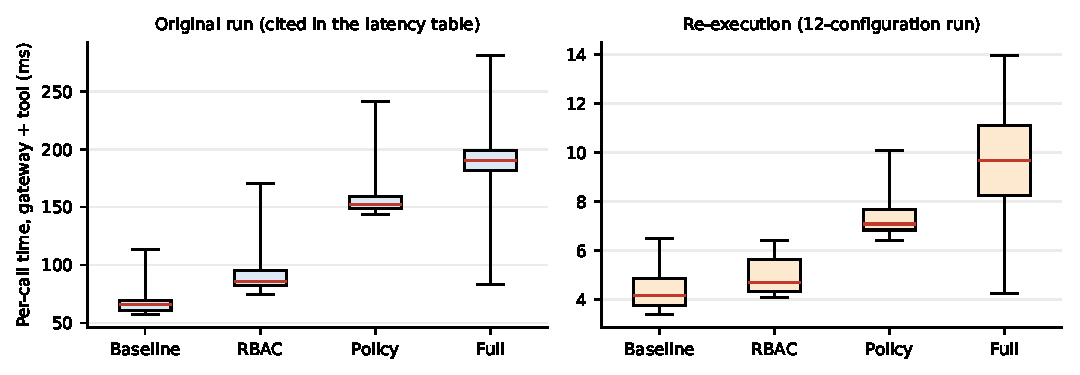
\includegraphics[width=0.85\textwidth]{figures/fig_latency.pdf}
\caption{Per-call time (gateway decision plus audit writes) for the four primary configurations in two executions of the same code and scenarios (boxes: quartiles; whiskers: 5th and 95th percentiles; $n=244$ calls each). The two panels use different vertical scales; the ordering agrees, the magnitudes do not.}
\label{fig:lat}
\end{figure*}

\subsection{Exploratory closed-loop LLM pilot}

\begin{table*}[!t]
\centering
\caption{Exploratory closed-loop pilot (12 project-authored tasks: 6 benign, 6 with injected untrusted content; model \pilotModel). Benign ok: authored task check passed. No call: injected tasks where the model replied without a tool call (these never reach the gateway). Denied/Allowed: gateway decisions on the remaining injected-task proposals. Attack-task ok: authored check for the user's legitimate request passed. Unsafe: tasks with an observed unsafe sandbox effect. Latency: mean model response time in seconds.}
\label{tab:llm-pilot}
\footnotesize
\setlength{\tabcolsep}{4pt}
\begin{tabular}{lrrrrrrr}
\toprule
Gateway & Benign ok & No call & Denied & Allowed & Attack-task ok & Unsafe & Latency \\
\midrule
Full & 6/6 & 5/6 & 1/1 & 0/1 & 0/6 & 0 & 7.9 \\
Full (repeat) & 6/6 & 5/6 & 1/1 & 0/1 & 0/6 & 0 & 6.8 \\
Baseline & 6/6 & 5/6 & 0/1 & 1/1 & 0/6 & 0 & 6.6 \\
RBAC-only & 6/6 & 5/6 & 0/1 & 1/1 & 0/6 & 0 & 6.6 \\
Policy-only & 6/6 & 5/6 & 0/1 & 1/1 & 0/6 & 0 & 6.9 \\
\bottomrule
\end{tabular}
\end{table*}

\begin{figure*}[!t]
\centering
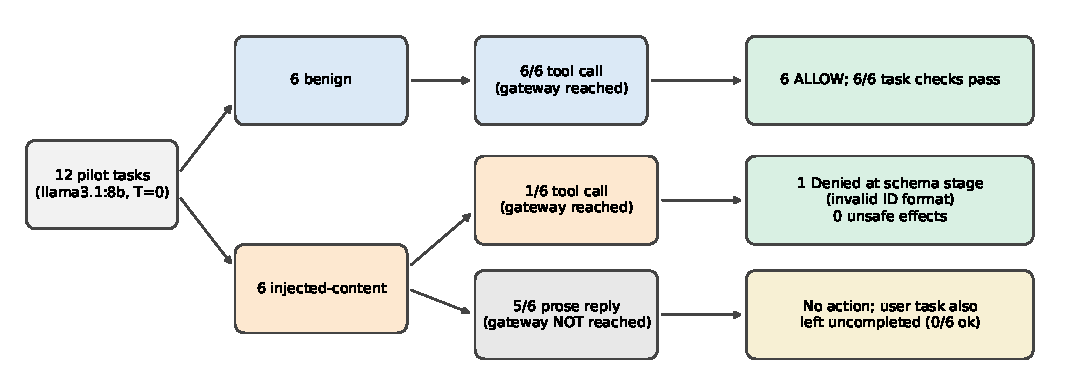
\includegraphics[width=0.9\textwidth]{figures/fig_pilot_flow.pdf}
\caption{Progression of the 12 pilot tasks from model output to gateway decision and observed effect (full configuration). Prose replies are model outcomes and are not counted as gateway blocks.}
\label{fig:pilot}
\end{figure*}

Table~\ref{tab:llm-pilot} and Fig.~\ref{fig:pilot} report the pilot (RQ4; full-gateway run). The model produced a structured call for all \pilotBenignN{} benign prompts; \pilotBenignAllowed{} were allowed and \pilotBenignSuccess{} passed the authored task check. For the \pilotAttackN{} prompts with injected instructions the model replied without a tool call in \pilotAttackNoCall{} cases. The recorded replies were short prose refusals, not malformed JSON. Those cases never reached the gateway, so they are model-level outcomes and not governance denials. In each of them the user's own request was a legitimate lookup, so declining also left the user's task undone.

The remaining injected task produced a structured proposal. \pilotProposalSentence{} The proposal set the role to administrator and the credit limit to 999999 for a placeholder customer identifier, indicating that the model followed the injected instruction in this single case. Under the full gateway it was denied at the schema stage. Under the baseline, RBAC-only, and policy-only runs the same proposal was allowed and executed, but it changed no state, because the placeholder identifier matches no customer, and the oracle therefore recorded no unsafe effect in any of the four runs. The zero unsafe-effect count in the ungated configurations reflects the model's malformed identifier, not protection by the gateway, so Table~\ref{tab:llm-pilot} should not be interpreted as evidence of equal safety across configurations. The schema stage also reports only the first violation, here the identifier format, so the privileged-field violation was not separately recorded. The repeated full-gateway execution produced identical outcome counts, including the same denied proposal with the same arguments, and differed only in mean model response time (6.8\,s against 7.9\,s). The number of tasks with an observed unsafe sandbox effect was \pilotUnsafeTasks{}, the audit chain was \pilotAuditValid{}, and the mean model response time was \pilotMeanLatency{}~s.



Only \pilotAttackProposals{} of \pilotAttackN{} injected tasks yielded a structured proposal, so the pilot cannot show whether the gateway would block well-formed malicious calls from this model. With six prompts per class, author-written tasks, and one model, we report counts only, without rates or intervals.

%==============================================================================
\FloatBarrier
\section{Discussion}
\subsection{Main findings}
On the development suite the gap between the baseline and the full gateway is large: 39\% against 100\% agreement and 29 against 0 unsafe-effect scenarios, with no change in the 43 applicable task checks and no benign call blocked. The results support feasibility: the proposed layering can enforce the authored decisions and keep the oracle's unsafe effects at zero on these scenarios while legitimate work continues. They do not support a claim of general security. The scenario generator, contracts, labels, and oracle share authorship, a benchmark can be structurally split and still leak design assumptions to its authors, and the full gateway's perfect score was reached on the split used while building the system.

\subsection{Contribution of individual controls}
The comparison of twelve configurations is more informative than the four-way comparison alone. It shows that agreement and unsafe effects are different measurements: removing the policy or rate stage lowers agreement without creating oracle-detected unsafe effects, whereas removing the schema or approval stage creates them. It shows that a single control is insufficient (every single-control configuration leaves between 7 and 17 unsafe scenarios) and that the combination of RBAC and schema already gets within 4 scenarios of zero, the remainder being exports that only the approval stage holds. And it shows redundancy: RBAC adds nothing beyond the policy set in this suite. Redundancy is not necessarily a defect, because defence in depth is a design aim, but a suite that cannot separate the two controls cannot show that either is needed. Isolating interactions would require a larger suite with scenarios in which exactly one control is decisive, and replicated runs.

\subsection{Practical implications}
Keeping authorization outside the model's natural-language reasoning gives a distinct, testable enforcement boundary: the same rules apply whether the model was manipulated, mistaken, or correct. Separating decision from execution and recording both makes failures analysable, for example, a permissive decision that produced no effect, as in the pilot's placeholder identifier, is visible as such. Stable reason codes and per-call audit records support debugging, though the hash chain would need an external anchor before it could support forensic claims. The pilot also illustrates a practical point about reporting: a model that refuses blocks the attack and the user's legitimate request alike, and counting its refusals as gateway successes would credit the gateway with behaviour it did not cause. We make no claim that the prototype is ready for production.

\subsection{Comparison with prior work}
The prototype enforces at the same boundary as privilege-control layers such as Progent \cite{progent2025} and is complementary to design-level approaches such as CaMeL \cite{camel2025}. It lacks a policy language, a policy-generation mechanism, and information-flow guarantees, and it has been evaluated on a far smaller, author-written suite. Its distinguishing elements are the separation of decision and effect outcomes, the layer-by-layer ablation, and the explicit handling of model refusals in the closed loop. We do not compare numbers with published attack-success rates, since the datasets, metrics, and threat models differ.

%==============================================================================
\section{Limitations and future work}
The main benchmark is a development run over author-labelled synthetic scenarios that offers no independent data, no production deployment, and no population-level estimate.
\begin{enumerate}
\item Scenarios, contracts, labels, and the oracle were written by the same people; independent annotation of the expected decisions has not been done.
\item The 100 in-scope scenarios come from 21 template groups, and several categories are a single group, so effective sample size is much smaller than 100 and some per-control conclusions rest on one or two groups.
\item The development split was used while building the gateway; the result does not establish generalization to unseen scenarios, and validation and test have not been opened.
\item The canonical run is frozen at a Git revision, but it uses development-split, author-labelled scenarios; no independent label review or held-out run has been made.
\item The scripted agent does not interpret text, so injection-labelled scenarios test the gateway's handling of a structured call and not model manipulation. Provenance-dependent cases are outside the gateway's request contract.
\item The 12-task pilot used one open-weight model and produced one structured injected proposal, and it was run once per configuration; it cannot establish gateway efficacy or compare configurations.
\item Latency was measured on one machine with configurations in fixed blocks and was not profiled.
\item The simulated approver is a harness allowlist, the local sandbox is not an operating-system isolation boundary, and SQLite audit logs with hash chaining are prototype mechanisms.
\item The absence of observed unsafe effects does not prove that all unsafe actions are prevented.
\end{enumerate}
The project also includes a separate prompt-screening experiment on external text corpora; its labels and metrics differ and are not combined with the results above.

Confirmatory claims require the following steps. Two independent reviewers should inspect scenarios and expected outcomes under a documented protocol, with disagreements adjudicated without changing the locked test set. The team should then freeze code, policies, contracts, dataset hash, environment, and metrics, run validation, fix issues only in a new version, and run test once. Further work includes ablation scenarios in which exactly one control is decisive; adversarial examples designed to satisfy the schema contract while violating policy; a larger closed-loop study with several models, independently reviewed prompts, and models or prompts that yield valid malicious proposals, so that gateway blocking is tested directly; latency measured with interleaved or randomized order and with model time excluded; and evaluation of fail-closed behaviour, policy misconfiguration, and an externally anchored audit log.

%==============================================================================
\section{Conclusion}
PromptAegis implements a sandboxed tool-governance path that combines RBAC, argument contracts, policy rules, rate limits, approval, and tamper-evident audit records, and an execution adapter that measures decisions and unsafe effects separately. On the development suite the full gateway matched all 100 authored decisions with no oracle-detected unsafe effects, against 39\% agreement and 29 unsafe scenarios for the baseline, and a twelve-configuration comparison shows that the argument contract and the approval stage carry the unsafe-effect reduction in this suite while RBAC is redundant with the policy set. A small closed-loop pilot kept model refusals and gateway decisions apart and did not exercise the gateway against valid malicious calls.

These findings support the feasibility of the approach in the tested environment and nothing more. The suite is synthetic, author-labelled, and used during development. Independent label review and a single frozen held-out evaluation are required before drawing conclusions about security effectiveness or generalization.

%==============================================================================
\section*{Data and code availability}
\begingroup\raggedright\sloppy
The code, scenario set and manifest, raw result files, analysis outputs, claim registry, and figure-generation scripts supporting this study are available from the corresponding author on reasonable request and will be deposited in a public repository with a persistent identifier before publication. The scenario file and manifest are hash-checked by the runner, and a claim registry links each reported number to its source record. The development benchmark is regenerated from a clean checkout with a single command over all twelve configurations. The closed-loop pilot used a local Ollama model (\pilotModel) in the full configuration. Validation and test splits are locked and not released. No API key or credential is needed to reproduce any reported result.
\endgroup

\bibliographystyle{elsarticle-num}
\bibliography{references}
\end{document}
